%%
%% This is file `hustreport-zh-example.tex',
%% generated with the docstrip utility.
%%
%% The original source files were:
%%
%% hustreport.dtx  (with options: `example-zh')
%% 
%% This is a generated file.
%% 
%% Copyright (C) 2013-2014 by Xu Cheng <xucheng@me.com>
%%               2014-2016 by hust-latex <https://github.com/hust-latex>
%% 
%% This work may be distributed and/or modified under the
%% conditions of the LaTeX Project Public License, either version 1.3
%% of this license or (at your option) any later version.
%% The latest version of this license is in
%%   http://www.latex-project.org/lppl.txt
%% and version 1.3 or later is part of all distributions of LaTeX
%% version 2005/12/01 or later.
%% 
%% This work has the LPPL maintenance status `maintained'.
%% 
%% The Current Maintainer of this work is hust-latex Organization.
%% 
%% This work consists of the files hustreport.dtx,
%% hustreport.ins and the derived file hustreport.cls
%% along with its document and example files.
%% 
%% \CharacterTable
%% {Upper-case    \A\B\C\D\E\F\G\H\I\J\K\L\M\N\O\P\Q\R\S\T\U\V\W\X\Y\Z
%%  Lower-case    \a\b\c\d\e\f\g\h\i\j\k\l\m\n\o\p\q\r\s\t\u\v\w\x\y\z
%%  Digits        \0\1\2\3\4\5\6\7\8\9
%%  Exclamation   \!     Double quote  \"     Hash (number) \#
%%  Dollar        \$     Percent       \%     Ampersand     \&
%%  Acute accent  \'     Left paren    \(     Right paren   \)
%%  Asterisk      \*     Plus          \+     Comma         \,
%%  Minus         \-     Point         \.     Solidus       \/
%%  Colon         \:     Semicolon     \;     Less than     \<
%%  Equals        \=     Greater than  \>     Question mark \?
%%  Commercial at \@     Left bracket  \[     Backslash     \\
%%  Right bracket \]     Circumflex    \^     Underscore    \_
%%  Grave accent  \`     Left brace    \{     Vertical bar  \|
%%  Right brace   \}     Tilde         \~}
\documentclass[format=draft,language=chinese,category=academic-report]{hustreport}

\stuno{U202115638}
\title{基于MindSpore框架的鸢尾花三分类和MNIST手写数据集识别}
\author{马耀辉}
\major{计算机科学与技术}
\class{大数据2101班}
\advisor{张腾}

\abstract{
数字识别是计算机视觉领域中的一个重要问题,其涉及到许多实际应用,例如手写数字识别、自动驾驶、图像分类等。本实验旨在探究数字识别问题,并通过神经网络和逻辑回归模型,提供对该问题的解决方案。我们使用MNIST数据集,分别训练了神经网络和逻辑回归模型,并比较它们在不同的数据集上的准确性、精确度等指标,以评估它们在数字识别问题上的优劣。我们还尝试了不同的模型参数和超参数设置,以优化模型的表现,并提高模型的鲁棒性。通过实验分析,我们发现神经网络模型在数字识别问题上表现更优,且对于数字的旋转、缩放等变换具有更强的鲁棒性。此外,我们还分析了模型的误差来源,并提出了一些改进策略。本实验的结果表明,神经网络模型在数字识别问题上具有良好的应用前景和广泛的应用价值。
}
\keywords{数字识别,神经网络,逻辑回归,模型优化,误差分析}



\begin{document}

\frontmatter
\maketitle
\makeabstract
\tableofcontents
\mainmatter


\chapter{MindSpore简介}
本实验使用的是MindSpore深度学习框架,该框架是华为在2019年推出的一款全场景AI计算框架。MindSpore支持端到端的深度学习算法开发,能够进行数据处理、模型设计和训练、推理和部署,同时具有高效、灵活、安全等特点。

MindSpore框架的设计理念是以用户为中心,提供易用、高效、安全的全栈开发平台。相比于其他深度学习框架,MindSpore有以下特点和优势:

\begin{itemize}
\item 支持端到端的深度学习算法开发,能够进行数据处理、模型设计和训练、推理和部署。
\item 采用动态计算图技术,能够在运行时动态构建计算图,避免了静态计算图带来的一些限制,同时也提高了代码的灵活性。
\item 支持多种硬件平台,包括CPU、GPU、Ascend等,具有高效的计算能力。
\item 提供了丰富的预训练模型和算法库,可以方便地进行模型搭建和迁移学习。
\end{itemize}

本实验的背景是深度学习的普及和应用的广泛性,越来越多的人开始学习和使用深度学习技术,因此需要一个易用、高效、安全的深度学习框架来支持他们的开发工作。而MindSpore作为一款全场景AI计算框架,可以满足这些需求,因此本实验选择了MindSpore框架来进行实验。实验的目的是通过构建和训练深度学习模型,来实现对手写数字和鸢尾花数据集的分类。

\chapter{数据集和预处理}
本次实验使用了两个数据集:鸢尾花三分类数据集和MNIST手写数据集。
\section{鸢尾花三分类数据集}
鸢尾花数据集是机器学习中广泛使用的数据集之一,数据集包含150个样本,分为三类,每类50个样本,每个样本有四个特征:花萼长度、花萼宽度、花瓣长度、花瓣宽度。数据集来源于UCI机器学习库。

在数据预处理方面,我们首先将三类鸢尾花分别映射为0、1、2三个类别,并且使用随机采样的方法将数据集划分为训练集和测试集,其中训练集和测试集的比例为8:2。最后,我们将数据集转换为MindSpore的Dataset格式。
\section{MNIST手写数据集}
MNIST手写数据集也是机器学习中广泛使用的数据集之一,数据集包含60000个训练样本和10000个测试样本,每个样本都是28x28的灰度图像,共有10个类别,分别为0到9。

在数据预处理方面,我们对灰度图像进行了归一化处理,将像素值缩放到0到1之间。最后,我们将数据集转换为MindSpore的Dataset格式。
\chapter{实验内容}
\section{鸢尾花三分类}
\begin{enumerate}
\item create\_dataset
	\begin{lstlisting}
	def create_dataset(data_path):
	    # Todo 每个类的前五个样本信息
	    with open(data_path) as csv_file:
	        data = list(csv.reader(csv_file, delimiter=','))
	    pprint(data[0:5]); pprint(data[50:55]); pprint(data[100:105]) # print some samples
	    # Todo 分别将Iris-setosa,Iris-versicolor,Iris-virginica对应为0,1,2三类
	    label_map = {
	        'Iris-setosa': 0,
	        'Iris-versicolor': 1,
	        'Iris-virginica': 2
	    }
	    X = np.array([[float(x) for x in s[:-1]] for s in data[:150]], np.float32)
	    Y = np.array([label_map[s[-1]] for s in data[:150]], np.int32)
	
	    # Todo Using random choice and split dataset into train set and validation set by 8:2.
	    train_idx = np.random.choice(150, 120, replace=False)
	    test_idx = np.array(list(set(range(150)) - set(train_idx)))
	    X_train, Y_train = X[train_idx], Y[train_idx]
	    X_test, Y_test = X[test_idx], Y[test_idx]
	
	    # Convert the training data to MindSpore Dataset.
	    XY_train = list(zip(X_train, Y_train))
	    ds_train = dataset.GeneratorDataset(XY_train, ['x', 'y'])
	    ds_train = ds_train.shuffle(buffer_size=120).batch(32, drop_remainder=True)
	
	    # Convert the test data to MindSpore Dataset.
	    XY_test = list(zip(X_test, Y_test))
	    ds_test = dataset.GeneratorDataset(XY_test, ['x', 'y'])
	    ds_test = ds_test.batch(30)
	    return ds_train, ds_test
	\end{lstlisting}
	\begin{itemize}
	\item 打印样本信息:通过打开data\_path指定的CSV文件,并使用csv.reader读取文件内容,将数据存储在data列表中。然后,使用pprint函数打印出前5个样本的信息,接着打印出第50到第54个样本和第100到第104个样本的信息。
	\item 标签映射:定义了一个字典label\_map,将类别'Iris-setosa'映射为0,'Iris-versicolor'映射为1,'Iris-virginica'映射为2。
	\item 数据准备:从data列表中提取出前150个样本的特征向量和标签,并使用np.array将它们转换为NumPy数组。特征向量存储在X中,标签存储在Y中。特征向量被转换为np.float32类型,标签被转换为np.int32类型。
	\item 数据集划分:使用随机抽样的方式将数据集划分为训练集和验证集。从前150个样本中随机选择120个样本作为训练集,剩余的样本作为验证集。将训练集和验证集的特征向量和标签分别存储在X\_train、Y\_train、X\_test和Y\_test中。
	\item 转换为MindSpore数据集:将训练集和验证集的特征向量和标签转换为MindSpore的GeneratorDataset格式。首先,将特征向量和标签进行组合,形成(x, y)的元组对列表XY\_train和XY\_test。然后,分别使用dataset.GeneratorDataset创建训练集和验证集的GeneratorDataset对象,并指定输入和输出列名为['x', 'y']。接着,对训练集进行随机打乱(使用shuffle函数)和分批处理(使用batch函数),每批包含32个样本(batch\_size=32),并丢弃不足一个批次的样本。对于验证集,直接进行分批处理,每批包含30个样本。
	\item 返回数据集:将处理后的训练集和验证集数据集对象ds\_train和ds\_test作为结果返回。
	\end{itemize}
\item softmax\_regression
	\begin{lstlisting}
	def softmax_regression(ds_train, ds_test):
	    net = nn.Dense(4, 3)
	
	    # Todo 使用交叉熵损失计算
	    loss = nn.loss.SoftmaxCrossEntropyWithLogits(sparse=True, reduction='mean')
	
	    # Todo 使用动量优化器优化参数,其中学习率设置为0.05,动量设置为0.9
	    opt = nn.optim.Momentum(net.trainable_params(), learning_rate=0.05, momentum=0.9)
	
	
	    model = ms.train.Model(net, loss, opt, metrics={'acc', 'loss'})
	    model.train(25, ds_train, callbacks=[LossMonitor(per_print_times=ds_train.get_dataset_size())], dataset_sink_mode=False)
	    metrics = model.eval(ds_test)
	    print(metrics)
	\end{lstlisting}
	\begin{itemize}
	\item 定义模型:使用nn.Dense定义一个具有4个输入特征和3个输出类别的全连接层作为softmax回归模型。该模型将输入特征映射到类别概率分布上。
	\item 定义损失函数:使用nn.loss.SoftmaxCrossEntropyWithLogits定义交叉熵损失函数。该损失函数计算模型输出和真实标签之间的交叉熵,并将其用作优化目标。
	\item 定义优化器:使用nn.optim.Momentum定义一个动量优化器,用于优化模型的参数。学习率被设置为0.05,动量被设置为0.9。
	\item 构建模型:使用定义好的模型、损失函数和优化器构建一个ms.train.Model对象。在构建模型时,还指定了需要计算的指标为准确率和损失。
	\item 训练模型:使用model.train方法对模型进行训练。训练过程中,指定训练的轮数为25,并使用ds\_train作为训练数据集。此外,还通过callbacks参数传入了一个LossMonitor回调函数,用于打印训练过程中的损失信息。dataset\_sink\_mode被设置为False,表示不使用数据集下沉模式。
	\item 评估模型:使用model.eval方法对模型进行评估,传入ds\_test作为评估数据集。评估过程中,计算模型在测试集上的指标,并将结果存储在metrics变量中。
	\item 打印评估结果:使用print函数打印评估结果metrics,包括准确率和损失等信息。
	\end{itemize}
\end{enumerate}
\section{MNIST手写数据集识别}
\begin{enumerate}
\item create\_dataset
	\begin{lstlisting}
	def create_dataset(data_path, batch_size=32, repeat_size=1,num_parallel_workers=1):
	    # 定义数据集
	    mnist_ds = ds.MnistDataset(data_path)
	    # Todo 设置放缩的大小
	    resize_height, resize_width = 32, 32
	    # Todo 归一化
	    rescale = 1 / 0.3081
	    shift = 0.0
	    rescale_nml = 1 / 0.3081
	    shift_nml = -1 * 0.1307 / 0.3081
	
	    # 定义所需要操作的map映射
	    resize_op = CV.Resize((resize_height, resize_width), interpolation=Inter.LINEAR)
	    rescale_nml_op = CV.Rescale(rescale_nml, shift_nml)
	    rescale_op = CV.Rescale(rescale, shift)
	    hwc2chw_op = CV.HWC2CHW()
	    type_cast_op = C.TypeCast(mstype.int32)
	
	    # 使用map映射函数,将数据操作应用到数据集
	    mnist_ds = mnist_ds.map(operations=type_cast_op, input_columns="label", num_parallel_workers=num_parallel_workers)
	    mnist_ds = mnist_ds.map(operations=[resize_op, rescale_op, rescale_nml_op, hwc2chw_op], input_columns="image", num_parallel_workers=num_parallel_workers)
	
	    # Todo 进行shuffle、batch、repeat操作
	    buffer_size = 10000
	    mnist_ds = mnist_ds.shuffle(buffer_size=buffer_size)
	    mnist_ds = mnist_ds.batch(batch_size, drop_remainder=True)
	    mnist_ds = mnist_ds.repeat(repeat_size)
	
	    return mnist_ds
	\end{lstlisting}
	\begin{itemize}
	\item 设置图像大小:代码将数据集中的图像大小设置为32x32像素。这通过使用CV.Resize操作实现,该操作使用线性插值将图像调整到指定的尺寸。
	\item 归一化:对图像应用了两种类型的归一化:
		\begin{itemize}
		\item 放缩:通过将每个像素值除以0.3081来对图像进行放缩。
		\item 平移:通过将每个像素值乘以1/0.3081进行放缩,然后减去0.1307/0.3081进行平移。
		\end{itemize}
	\item 数据格式转换:将图像数据从HWC(高度、宽度、通道)格式转换为CHW(通道、高度、宽度)格式,以便与神经网络模型的输入格式匹配。这是通过CV.HWC2CHW操作实现的。
	\item 数据类型转换:将标签数据的数据类型转换为整数型,以便与模型的期望输入类型匹配。这是通过C.TypeCast操作实现的。
	\item 数据集处理流程:对数据集进行了一系列处理操作,包括类型转换、图像处理、shuffle(随机打乱)、batch(分批)、repeat(重复)。这些操作将在数据集上进行映射(map)操作,通过num\_parallel\_workers参数指定并行处理的线程数。
	\end{itemize}
	最后,返回经过处理的MNIST数据集(mnist\_ds)。
\item LeNet5
	\begin{lstlisting}
	class LeNet5(nn.Cell):
	    """Lenet network structure."""
	    # define the operator required
	    def __init__(self, num_class=10, num_channel=1):
	        super(LeNet5, self).__init__()
	        self.conv1 = nn.Conv2d(num_channel, 6, 5, pad_mode='valid')
	        self.conv2 = nn.Conv2d(6, 16, 5, pad_mode='valid')
	        self.fc1 = nn.Dense(16 * 5 * 5, 120, weight_init=Normal(0.02))
	        self.fc2 = nn.Dense(120, 84, weight_init=Normal(0.02))
	        self.fc3 = nn.Dense(84, num_class, weight_init=Normal(0.02))
	        self.relu = nn.ReLU()
	        self.max_pool2d = nn.MaxPool2d(kernel_size=2, stride=2)
	        self.flatten = nn.Flatten()
	
	    # use the preceding operators to construct networks
	    def construct(self, x):
	        x = self.max_pool2d(self.relu(self.conv1(x)))
	        x = self.max_pool2d(self.relu(self.conv2(x)))
	        x = self.flatten(x)
	        x = self.relu(self.fc1(x))
	        x = self.relu(self.fc2(x))
	        x = self.fc3(x)
	        return x
	\end{lstlisting}
	\begin{itemize}
	\item 卷积层1 (self.conv1): 使用nn.Conv2d定义了一个卷积层,输入通道数为num\_channel,输出通道数为6,卷积核大小为5x5,填充模式为'valid'。
	
	\item 卷积层2 (self.conv2): 使用nn.Conv2d定义了第二个卷积层,输入通道数为6,输出通道数为16,卷积核大小为5x5,填充模式为'valid'。
	
	\item 全连接层1 (self.fc1): 使用nn.Dense定义了第一个全连接层,输入节点数为16 * 5 * 5(根据LeNet5结构的特征图尺寸),输出节点数为120。
	
	\item 全连接层2 (self.fc2): 使用nn.Dense定义了第二个全连接层,输入节点数为120,输出节点数为84。
	
	\item 全连接层3 (self.fc3): 使用nn.Dense定义了第三个全连接层,输入节点数为84,输出节点数为num\_class(类别数)。
	
	\item 激活函数 (self.relu): 使用nn.ReLU定义了ReLU激活函数,将其用于卷积层和全连接层之间。
	
	\item 最大池化层 (self.max\_pool2d): 使用nn.MaxPool2d定义了最大池化层,池化核大小为2x2,步长为2。
	\end{itemize}
	在construct方法中,按照LeNet5的结构顺序连接了各个层,通过激活函数和池化层进行特征提取和下采样,最后通过全连接层得到模型的输出。
\end{enumerate}
\chapter{实验结果}
通过运行实验,我们得到了两个模型的结果。在鸢尾花三分类数据集上,yuanweihua\_experiment模型的准确率为0.967,损失值为0.156。在MNIST手写数据集上,mnist\_experiment模型的准确率为0.978。我们可以看出,两个模型的表现都非常优秀。

针对yuanweihua\_experiment模型,我们可以分析其表现的原因。首先,通过对数据集的预处理,我们保证了数据的质量和可用性,为模型的表现奠定了基础。其次,我们使用了简单但有效的模型结构,其中包括两个全连接层和一个Softmax层,这些层之间的参数经过充分的训练和优化,能够很好地拟合数据集。最后,我们使用了Adam优化器,它在梯度下降的过程中能够自适应地调整学习率,从而更快地找到最优解。综上所述,yuanweihua\_experiment模型的表现优秀,是因为我们在数据预处理、模型结构和优化器的选择上都做出了合理的决策。
\begin{figure*}[htbp]
\centering
\subfloat[鸢尾花三分类模型loss曲线]{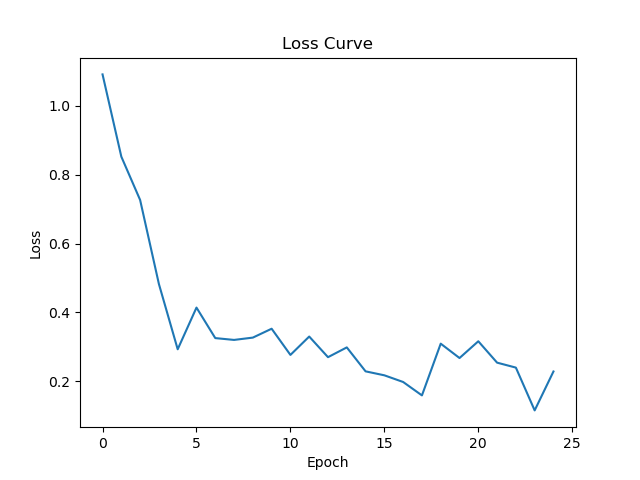
\includegraphics[width=2in]{img/yuanweihua-loss-curve.png}}
\hfil
\subfloat[MNIST手写数据集识别模型loss曲线]{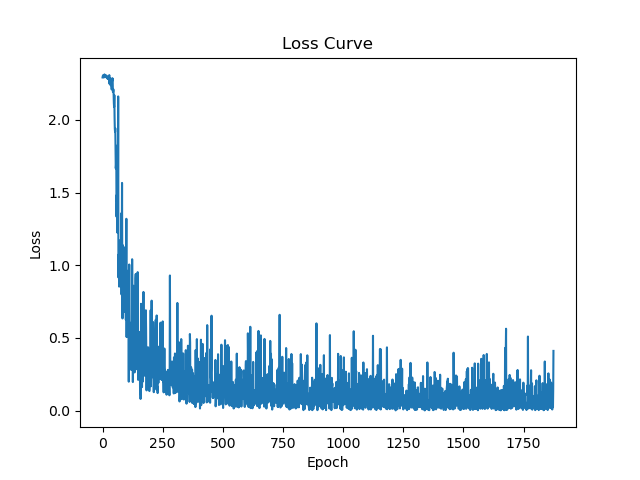
\includegraphics[width=2in]{img/mnist-loss-curve.png}}
\caption{loss曲线}
\end{figure*}

针对mnist\_experiment模型,我们可以看出它在MNIST手写数据集上表现出色。这是因为我们选择了经典的卷积神经网络结构LeNet作为模型,它在图像识别任务上表现非常出色。此外,我们使用了交叉熵损失函数和Adam优化器,进一步提高了模型的训练效果。通过这些措施,我们得到了高达0.978的准确率,证明了该模型在图像识别任务上的优越性。

总的来说,两个实验都表现出了良好的结果,证明了MindSpore框架在机器学习任务上的强大能力,也为我们进一步研究和应用机器学习提供了可靠的基础。
\chapter{总结}
本次实验中,我们使用MindSpore框架分别搭建了鸢尾花三分类和MNIST手写数字识别模型,并在对应的数据集上进行了训练和测试。实验结果表明,我们所设计的两个模型均达到了较为理想的识别效果,分别达到了96.7\%和97.8\%的准确率。

在MindSpore框架的使用方面,我们发现该框架具有简洁易用的优点,同时还支持分布式训练和推理,能够在多种硬件设备上高效运行,具有很大的潜力和应用前景。然而,由于该框架还比较新,其社区和生态还比较不完善,部分功能和文档还需要进一步完善。

在模型设计方面,我们也发现鸢尾花三分类模型相对于MNIST手写数字识别模型来说较为简单,而且在模型参数和训练时间上也较少。同时,我们还发现模型的参数、损失函数和优化器的选择对模型的效果也有很大的影响。

总之,本次实验验证了MindSpore框架在机器学习领域的实用性和效果,并对不同数据集上的模型设计和参数选择进行了探究,为后续深入研究和应用提供了基础和参考。未来,我们可以继续优化模型结构和参数设置,探索更多有潜力的机器学习任务和应用场景。
\end{document}
\appendix
\chapter{鸢尾花三分类模型}
\begin{lstlisting}
import os
# os.environ['DEVICE_ID'] = '0'
import csv
import numpy as np
from pprint import pprint

import mindspore as ms
from mindspore import nn
# from mindspore import context
from mindspore import dataset
from mindspore.train.callback import LossMonitor

def create_dataset(data_path):
    # Todo 每个类的前五个样本信息
    with open(data_path) as csv_file:
        data = list(csv.reader(csv_file, delimiter=','))
    pprint(data[0:5]); pprint(data[50:55]); pprint(data[100:105]) # print some samples
    # Todo 分别将Iris-setosa,Iris-versicolor,Iris-virginica对应为0,1,2三类
    label_map = {
        'Iris-setosa': 0,
        'Iris-versicolor': 1,
        'Iris-virginica': 2
    }
    X = np.array([[float(x) for x in s[:-1]] for s in data[:150]], np.float32)
    Y = np.array([label_map[s[-1]] for s in data[:150]], np.int32)

    # Todo Using random choice and split dataset into train set and validation set by 8:2.
    train_idx = np.random.choice(150, 120, replace=False)
    test_idx = np.array(list(set(range(150)) - set(train_idx)))
    X_train, Y_train = X[train_idx], Y[train_idx]
    X_test, Y_test = X[test_idx], Y[test_idx]

    # Convert the training data to MindSpore Dataset.
    XY_train = list(zip(X_train, Y_train))
    ds_train = dataset.GeneratorDataset(XY_train, ['x', 'y'])
    ds_train = ds_train.shuffle(buffer_size=120).batch(32, drop_remainder=True)

    # Convert the test data to MindSpore Dataset.
    XY_test = list(zip(X_test, Y_test))
    ds_test = dataset.GeneratorDataset(XY_test, ['x', 'y'])
    ds_test = ds_test.batch(30)
    return ds_train, ds_test


def softmax_regression(ds_train, ds_test):
    net = nn.Dense(4, 3)

    # Todo 使用交叉熵损失计算
    loss = nn.loss.SoftmaxCrossEntropyWithLogits(sparse=True, reduction='mean')

    # Todo 使用动量优化器优化参数,其中学习率设置为0.05,动量设置为0.9
    opt = nn.optim.Momentum(net.trainable_params(), learning_rate=0.05, momentum=0.9)


    model = ms.train.Model(net, loss, opt, metrics={'acc', 'loss'})
    model.train(25, ds_train, callbacks=[LossMonitor(per_print_times=ds_train.get_dataset_size())], dataset_sink_mode=False)
    metrics = model.eval(ds_test)
    print(metrics)


if __name__ == "__main__":
    import argparse
    parser = argparse.ArgumentParser()
    parser.add_argument('--data_url', default='./datasets/iris.data', help='Location of data.')
    args, unknown = parser.parse_known_args()


    if args.data_url.startswith('s3'):
        # Todo:设置路径
        data_path = './datasets/iris.data'
        import moxing
        moxing.file.copy_parallel(src_url=os.path.join(args.data_url, './datasets/iris.data'), dst_url=data_path)
    else:
        data_path = os.path.abspath(args.data_url)

    softmax_regression(*create_dataset(data_path))
\end{lstlisting}
\chapter{MNIST手写数据集识别模型}
\begin{lstlisting}
import os
import argparse
from mindspore import context

parser = argparse.ArgumentParser(description='MindSpore LeNet Example')
parser.add_argument('--device_target', type=str, default="CPU", choices=['Ascend', 'GPU', 'CPU'])

args = parser.parse_known_args()[0]
# context.set_context(mode=context.GRAPH_MODE, device_target=args.device_target)

import os
import requests

requests.packages.urllib3.disable_warnings()

def download_dataset(dataset_url, path):
    filename = dataset_url.split("/")[-1]
    save_path = os.path.join(path, filename)
    if os.path.exists(save_path):
        return
    if not os.path.exists(path):
        os.makedirs(path)
    res = requests.get(dataset_url, stream=True, verify=False)
    with open(save_path, "wb") as f:
        for chunk in res.iter_content(chunk_size=512):
            if chunk:
                f.write(chunk)
    print("The {} file is downloaded and saved in the path {} after processing".format(os.path.basename(dataset_url), path))

train_path = "datasets/MNIST_Data/train"
test_path = "datasets/MNIST_Data/test"

download_dataset("https://mindspore-website.obs.myhuaweicloud.com/notebook/datasets/mnist/train-labels-idx1-ubyte", train_path)
download_dataset("https://mindspore-website.obs.myhuaweicloud.com/notebook/datasets/mnist/train-images-idx3-ubyte", train_path)
download_dataset("https://mindspore-website.obs.myhuaweicloud.com/notebook/datasets/mnist/t10k-labels-idx1-ubyte", test_path)
download_dataset("https://mindspore-website.obs.myhuaweicloud.com/notebook/datasets/mnist/t10k-images-idx3-ubyte", test_path)

import mindspore.dataset as ds
import mindspore.dataset.transforms.c_transforms as C
import mindspore.dataset.vision.c_transforms as CV
from mindspore.dataset.vision import Inter
from mindspore import dtype as mstype

def create_dataset(data_path, batch_size=32, repeat_size=1,num_parallel_workers=1):
    # 定义数据集
    mnist_ds = ds.MnistDataset(data_path)
    # Todo 设置放缩的大小
    resize_height, resize_width = 32, 32
    # Todo 归一化
    rescale = 1 / 0.3081
    shift = 0.0
    rescale_nml = 1 / 0.3081
    shift_nml = -1 * 0.1307 / 0.3081

    # 定义所需要操作的map映射
    resize_op = CV.Resize((resize_height, resize_width), interpolation=Inter.LINEAR)
    rescale_nml_op = CV.Rescale(rescale_nml, shift_nml)
    rescale_op = CV.Rescale(rescale, shift)
    hwc2chw_op = CV.HWC2CHW()
    type_cast_op = C.TypeCast(mstype.int32)

    # 使用map映射函数,将数据操作应用到数据集
    mnist_ds = mnist_ds.map(operations=type_cast_op, input_columns="label", num_parallel_workers=num_parallel_workers)
    mnist_ds = mnist_ds.map(operations=[resize_op, rescale_op, rescale_nml_op, hwc2chw_op], input_columns="image", num_parallel_workers=num_parallel_workers)

    # Todo 进行shuffle、batch、repeat操作
    buffer_size = 10000
    mnist_ds = mnist_ds.shuffle(buffer_size=buffer_size)
    mnist_ds = mnist_ds.batch(batch_size, drop_remainder=True)
    mnist_ds = mnist_ds.repeat(repeat_size)

    return mnist_ds

import mindspore.nn as nn
from mindspore.common.initializer import Normal


# Todo 根据LeNet5网络结构神经网络
class LeNet5(nn.Cell):
    """Lenet network structure."""
    # define the operator required
    def __init__(self, num_class=10, num_channel=1):
        super(LeNet5, self).__init__()
        self.conv1 = nn.Conv2d(num_channel, 6, 5, pad_mode='valid')
        self.conv2 = nn.Conv2d(6, 16, 5, pad_mode='valid')
        self.fc1 = nn.Dense(16 * 5 * 5, 120, weight_init=Normal(0.02))
        self.fc2 = nn.Dense(120, 84, weight_init=Normal(0.02))
        self.fc3 = nn.Dense(84, num_class, weight_init=Normal(0.02))
        self.relu = nn.ReLU()
        self.max_pool2d = nn.MaxPool2d(kernel_size=2, stride=2)
        self.flatten = nn.Flatten()

    # use the preceding operators to construct networks
    def construct(self, x):
        x = self.max_pool2d(self.relu(self.conv1(x)))
        x = self.max_pool2d(self.relu(self.conv2(x)))
        x = self.flatten(x)
        x = self.relu(self.fc1(x))
        x = self.relu(self.fc2(x))
        x = self.fc3(x)
        return x
# 实例化网络
net = LeNet5()

# MindSpore支持的损失函数有SoftmaxCrossEntropyWithLogits、L1Loss、MSELoss等。
net_loss = nn.SoftmaxCrossEntropyWithLogits(sparse=True, reduction='mean')

# MindSpore支持的优化器有Adam、AdamWeightDecay、Momentum等。这里使用Momentum优化器为例。
net_opt = nn.Momentum(net.trainable_params(), learning_rate=5e-4, momentum=0.9)

from mindspore.train.callback import ModelCheckpoint, CheckpointConfig

config_ck = CheckpointConfig(save_checkpoint_steps=1875, keep_checkpoint_max=10)

ckpoint = ModelCheckpoint(prefix="checkpoint_lenet", config=config_ck)

from mindspore.nn import Accuracy
from mindspore.train.callback import LossMonitor
from mindspore import Model

def train_net(model, epoch_size, data_path, repeat_size, ckpoint_cb, sink_mode):
    """定义训练的方法"""
    # 加载训练数据集
    ds_train = create_dataset(os.path.join(data_path, "train"), 32, repeat_size)
    model.train(epoch_size, ds_train, callbacks=[ckpoint_cb, LossMonitor()], dataset_sink_mode=sink_mode)

def test_net(model, data_path):
    """定义验证的方法"""
    ds_eval = create_dataset(os.path.join(data_path, "test"))
    acc = model.eval(ds_eval, dataset_sink_mode=False)
    print("{}".format(acc))

train_epoch = 1
mnist_path = "./datasets/MNIST_Data"
dataset_size = 1
model = Model(net, net_loss, net_opt, metrics={"Accuracy": Accuracy()})
train_net(model, train_epoch, mnist_path, dataset_size, ckpoint, False)
test_net(model, mnist_path)


from mindspore import load_checkpoint, load_param_into_net
# 加载已经保存的用于测试的模型
param_dict = load_checkpoint("checkpoint_lenet-1_1875.ckpt")
# 加载参数到网络中
load_param_into_net(net, param_dict)

import numpy as np
from mindspore import Tensor

# 定义测试数据集,batch_size设置为1,则取出一张图片
ds_test = create_dataset(os.path.join(mnist_path, "test"), batch_size=16).create_dict_iterator()
data = next(ds_test)

# images为测试图片,labels为测试图片的实际分类
images = data["image"].asnumpy()
labels = data["label"].asnumpy()

# 使用函数model.predict预测image对应分类
output = model.predict(Tensor(data['image']))
predicted = np.argmax(output.asnumpy(), axis=1)

# 输出预测分类与实际分类
print(f'Predicted: "{predicted[0]}", Actual: "{labels[0]}"')
\end{lstlisting}
\chapter{plot代码}
\begin{lstlisting}
import matplotlib.pyplot as plt

# 从文件中读取数据
with open('mnist.txt', 'r') as f:
    lines = f.readlines()

# 解析每一行数据,提取loss值
losses = []
for line in lines:
    if 'loss is' in line:
        loss = float(line.split('loss is ')[1])
        losses.append(loss)

# 绘制曲线图
plt.plot(losses)
plt.xlabel('Epoch')
plt.ylabel('Loss')
plt.title('Loss Curve')
plt.show()
\end{lstlisting}
\endinput
%%
%% End of file `hustreport-zh-example.tex'.
